\section{Konsept}
\label{sec:konsept}
%En overordnet beskrivelse av hva systemet skal gjøre. Her legges vekt på hvordan systemet skal oppføre seg, ikke hvordan det er designet.

Systemet som designes skal kartlegge og dokumentere aktiviteten av fugler. Det skal både kunne brukes i områder med vindturbiner allerede instalert og i områder hvor det planlegges eller vurderes å installere vindturbiner, hvor det ellers ville vært nødvendig å ansette ornitologer. Dette skal kunne gjøres på en billig og effektiv måte, kontinuerlig hele døgnet. Både antall fugler i området og når på døgnet det er mest aktivitet skal kunne fastslås. Konseptet er vist i \autoref{fig:konsept}.

%ny figur? illustrasjon av vindmølle med fugler og sensor, som gjør det den gjør, viser liksom situasjonen den brukes i og sånn
%dette vil medføre at figuren som nå er i konsept flyttes til design


\begin{figure}[H]
    \centering
    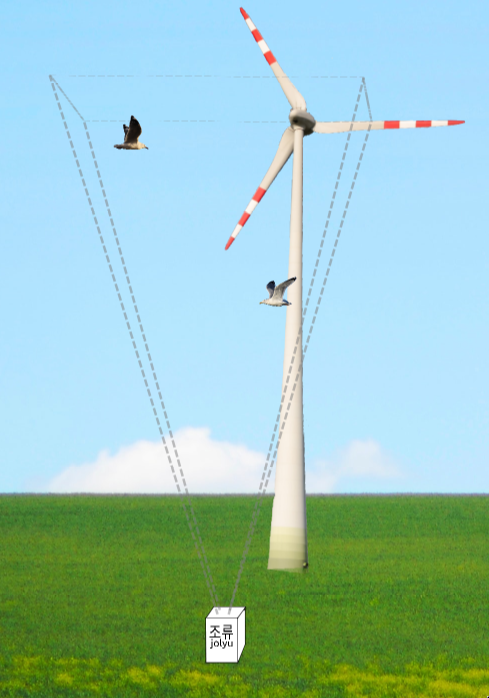
\includegraphics[width=0.5\textwidth]{konsept/KonseptBilde.png}
    \caption{Hvordan konseptet er tenkt å fungere. Et infrarødt kamera detekterer fugler som flyr i et område i luften. }
    \label{fig:konsept}
\end{figure}

%VELDIG lik den i implementasjon
%finnes fire versjoner

Deteksjonen skal foregå med et infrarødt kamera som kontinuerlig tar bilder av himmelen for å se etter varmesignaturer fra fugler. Bildene prosesseres, og varmesignaturen fra hver fugl spores fra bilde til bilde og loggføres. Alle fugler i bildet spores individuelt. Systemet skal også innhente grunnleggende værdata: nedbør, vind, vindretning, temperatur, luftfuktighet og lufttrykk. Data om fugleaktivitet og værforhold skal overføres trådløst og presenteres på en nettside.



%ting som skal addes:

%
%
%
%
%
%
%
%
%



%tekst fra innleveringen:
%Systemet skal være i stand til å kunne telle fugler som flyr over et gitt område. Fuglene på himmelen skal telles og loggføres, og spores på en slik måte at en passerende fugl kun telles én gang. Dette oppnås ved at et infrarødt kamera filmer himmelen og eventuelle fuglers varmesignatur mot himmelen. Bildene analyseres i en prosesseringsenhet, som oppdager og sporer fuglene. I tillegg skal systemet inneholde sensorer for å måle værdata. Dette inkluderer nedbør, luftfuktighet, temperatur, trykk, lys, og vind. Data overføres så trådløst til en nettside, hvor den fremstilles til brukere og kan analyseres videre. Systemet kan utvides med flere kameraer for økt dekning, eller flere separate enheter. Et økt dekningsområde gir større muligheter for avansert sporing eller overvåkning av fugleaktivitet, eller for å kunne observere forskjeller i aktivitet i sanntid.

